% !TEX encoding = UTF-8
% !TEX TS-program = pdflatex
% !TEX root = ../tesi.tex

%**************************************************************
\chapter{Analisi dei requisiti}
\label{cap:analisi-requisiti}
Il presente capitolo ha come scopo quello di fornire una descrizione completa e precisa di tutti i requisitiG individuati e dei casi d’uso ad alto livello riguardanti il progetto CS-Template.

\section{Casi d'uso}

Per lo studio dei casi di utilizzo del prodotto sono stati creati dei diagrammi.
I diagrammi dei casi d'uso (in inglese \emph{Use Case Diagram}) sono diagrammi di tipo \gls{UML} dedicati alla descrizione delle funzioni o servizi offerti da un sistema, così come sono percepiti e utilizzati dagli attori che interagiscono col sistema stesso.
Ogni caso d’uso è definito secondo la seguente struttura:
\begin{itemize}
	\item Nome: Il titolo del caso d’uso;
	\item Attori: Indica gli attori principali e secondari del caso d’uso. In tutto il contesto
	dell’applicazione gli autori del sistema saranno così classificati:
	\begin{itemize}
		\item Utente Zendesk: sono gli utenti della piattaforma Zendesk. Possono essere gli agenti(persone che gestiscono le richieste dei cleinti) oppure gli amministratore di Zendesk;
		\item Utente generico: utente qualsiasi che non ha ancora effettuato l'accesso alla pagina degli amministratori;
		 \item Amministratore: utente amministratore Nextep, che ha compito di gestire tutti le aziende che utilizzano l'applicazione CS-Template.
	\end{itemize}

	\item Descrizione: Riporta una breve descrizione del caso d’uso;
	\item Precondizione: Specifica le condizioni che sono identificate come vere prima
	del verificarsi degli eventi del caso d’uso;
	\item Postcondizione: Specifica le condizioni che sono identificate come vere dopo il
	verificarsi degli eventi del caso d’uso.

\end{itemize}

\subsection{ Casi d'uso pagina degli amministratori}
Questa è la pagina web il cui scopo principale è quello di visualizzare la lista di tutti i clienti di Nextep che hanno l'applicazione CS-Template installata sulla propria piattaforma Zendesk. Inoltre permette di aggiungerne dei nuovi. L'accesso a questa pagina è garantita solo agli uenti amministratori di Nextep con le credenziali valide.
\begin{usecase}{1}{Login pagina amministratori}

	\usecaseactors{Utente generico}
	\usecasedesc{Caso d'uso descrive login alla pagina degli amministratori. }
	\usecasepre{L'utente non autenticato}
	\usecasepost{Il sistema riconosce l'utente amministratore}
		\begin{figure}[!h] 
		\centering 
		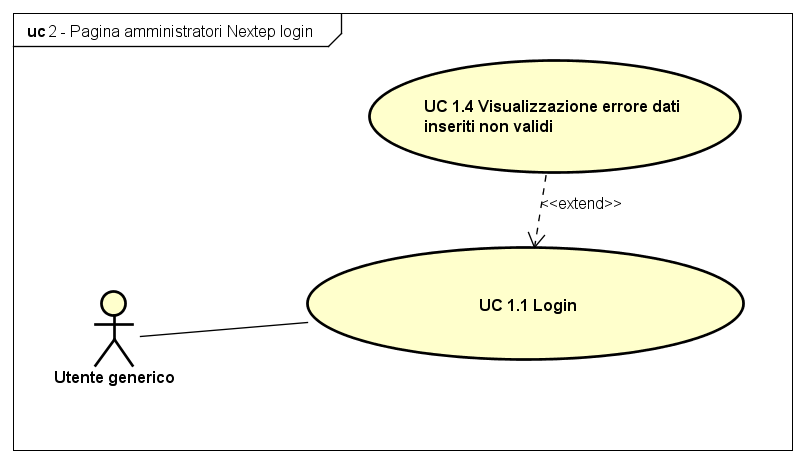
\includegraphics[width=1\columnwidth]{usecase/login} 
		\caption{UC 1 - pagina login}
	\end{figure}
\\ 
\\
\begin{usecase}{2}{Pagina degli amministratori}
	
	\usecaseactors{Nextep Admin}
	\usecasedesc{Caso d'uno descrive le funzionalità della pagina degli amministratori di Nextep. In questa pagina è possibile gestire tutti i clienti(aziende) di Nextep che utilizzano l'applicazione CS-Template}
	\usecasepre{Il sistema riconosce l'amministratore}
	\usecasepost{L’amministratore visualizza una lista di tutti i clienti(utilizzatori di CS-Template) registrati  nel  sistema,  visualizzando  per  ognuno  di  essi tutte le   informazioni  e un form per aggiungerne uno nuovo}
	\begin{figure}[!h] 
		\centering 
		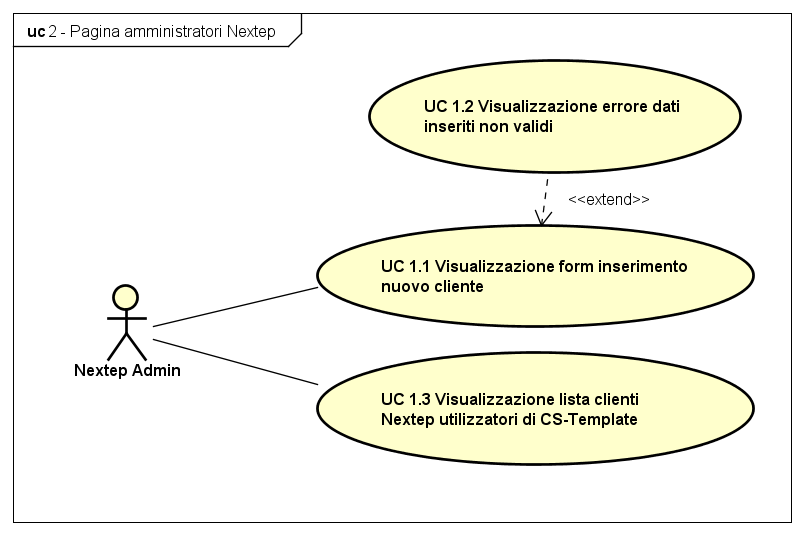
\includegraphics[width=1\columnwidth]{usecase/paginaAdmin} 
		\caption{UC 2 - funzionalità pagina admin}
	\end{figure}
\end{usecase}
\newpage
\subsection{ Casi d'uso pagina contenente l'editor drag-and-drop}
Questa pagina web contiene l'editor drag-and-drop che verrà visualizzato successivamente nella piattaforma Zendesk in un iframe. In seguito è riportato un caso d'uso generico che descrive tutte le proprietà ad alto livello dell'editor.
\begin{usecase}{3}{Editor drag-and-drop}
	
	\usecaseactors{Utente Zendesk}
	\usecasedesc{Caso d'uso descrive tutte le funzionalità ad alto livello che l'editor dovrà fornire}
	\usecasepre{L'utente Zendesk apre l'editor}
	\usecasepost{L'editor permette all'utente Zendesk di realizzare qualsiasi tipo di contentuto HTML e CSS}
	\begin{figure}[!h] 
		\centering 
		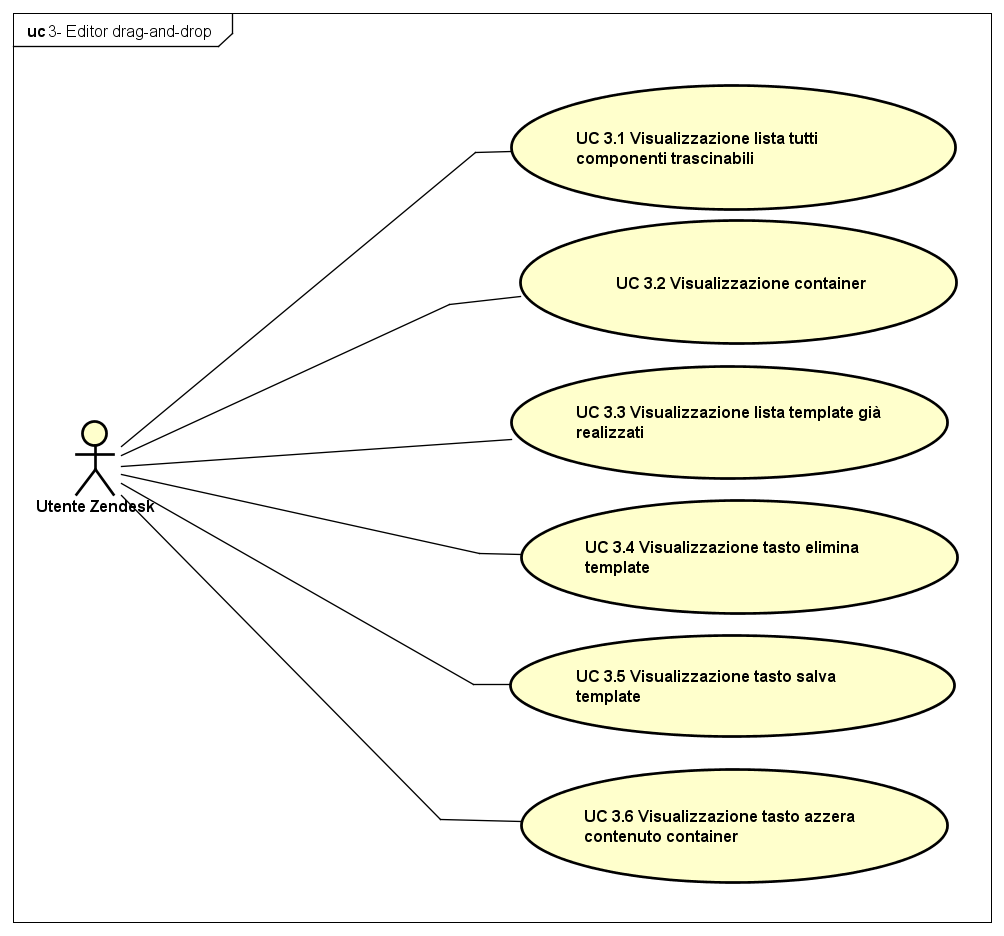
\includegraphics[width=1\columnwidth]{usecase/editor} 
		\caption{UC3 - pagina contenene l'editor}
	\end{figure}
\end{usecase}
\newpage
\subsection{ Casi d'uso pagina contenente il widget}
Questa pagina web contiene il widget che verrà visualizzato successivamente nella piattaforma Zendesk in un iframe. Il widget verrà mostrato quando verrà aperto una richeista qualsiasi del cliente. Esso permette di scegliere da una lista il contenuto HTML e CSS da utilizzare come risposta verso il cliente. 
\begin{usecase}{4}{Widget dei template}
	
	\usecaseactors{Utente Zendesk}
	\usecasedesc{Caso d'uso descrive tutte le funzionalità ad alto livello che il widget dovrà fornire}
	\usecasepre{L'utente Zendesk apre il widget}
	\usecasepost{Utente Zendesk sceglie il template da inviare come risposta al cliente}
	\begin{figure}[!h] 
		\centering 
		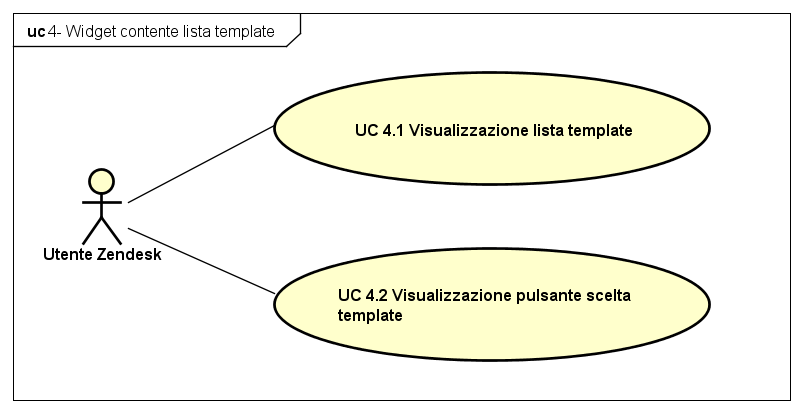
\includegraphics[width=1.2\columnwidth]{usecase/widget} 
		\caption{UC3 - pagina contenente il widget}
	\end{figure}
\\
\\
\\
\\
\\
\end{usecase}

\section{Tracciamento dei requisiti}

Da un'attenta analisi dei requisiti e degli use case effettuata sul progetto è stata stilata la tabella che traccia i requisiti in rapporto agli use case.\\
Sono stati individuati diversi tipi di requisiti e si è quindi fatto utilizzo di un codice identificativo per distinguerli.\\
Il codice dei requisiti è così strutturato R(F/V)(N/D) dove:
\begin{enumerate}
	\item[R =] requisito
    \item[F =] funzionale
    \item[V =] vincolo
    \item[N =] obbligatorio (necessario)
    \item[D =] desiderabile
\end{enumerate}

Nelle tabelle \ref{tab:requisiti-funzionali} e \ref{tab:requisiti-vincolo} sono riassunti i requisiti e il loro tracciamento con gli use case delineati in fase di analisi.
\\
\begin{table}%
\caption{Tabella del tracciamento dei requisti funzionali}
\label{tab:requisiti-funzionali}
\begin{tabularx}{\textwidth}{lXl}
\hline\hline
\textbf{Requisito} & \textbf{Descrizione} & \textbf{Use Case}\\
\hline
RFN-1   & Personale di Nextep può effetuare il login nella pagina degli amministraori & UC1 \\
\hline
RFN-2   & Nextep Admin può ottenere una lista con tutte le informazioni dei clienti che utilizzano l'applicazione CS-Template & UC2 \\
\hline
RFN-3   & Nextep Admin può eliminare un cliente dalla lista & UC2 \\
\hline
RFN-4   & Nextep Admin può aggiungere un nuovo cliente nella lista & UC2 \\
\hline
RFN-4   & Utente Zendesk può utilizzare l'editor drag-and-drop & UC3 \\
\hline
RFN-5   & Utente Zendesk può creare nuovi template & UC3 \\
\hline
RFN-6   & Utente Zendesk può salvare il template creato & UC3 \\
\hline
RFN-7   & Utente Zendesk può eliminare template creati & UC3 \\
\hline
RFN-8   & Utente Zendesk può azzerrare il contenuto del editor & UC3 \\
\hline
RFN-10   & Utente Zendesk può impostare il nome del template & UC3 \\
\hline
RFN-11   & Utente Zendesk può utilizzare il temaplte creato nella risposta verso il cliente & UC4 \\
\hline
RFD-12   & Utente Zendesk può esportare tutto i template creati in un file json come backup & UC4 \\
\hline
RFD-13   & Utente Zendesk può importare i template da un file json precedentemente creato & UC4 \\
\hline
\end{tabularx}
\end{table}%

\begin{table}%
\caption{Tabella del tracciamento dei requisiti di vincolo}
\label{tab:requisiti-vincolo}
\begin{tabularx}{\textwidth}{lXl}
\hline\hline
\textbf{Requisito} & \textbf{Descrizione} & \textbf{Use Case}\\
\hline
RVN-1    & Il backend dell'applicazioend deve essere realizzato utilizzando gli servizi cloud & - \\
\hline
RVN-2    & L'applicazione deve essere utilizzabile solo dai clienti aggiunti da Nextep, implementando un sistema d' accesso tramite il token & - \\
\hline
RVN-3    & L’intero progetto deve essere accompagnato da
documentazione completa & - \\
\hline
\end{tabularx}
\end{table}%